\documentclass[11pt,a4paper]{article}
\usepackage[utf8]{inputenc}
\usepackage[spanish]{babel}
\usepackage{graphicx}
\usepackage{geometry}
\usepackage{fancyhdr}
\usepackage{hyperref}
\usepackage{enumitem}
\usepackage{float}  % Paquete necesario para usar [H]

\geometry{margin=2.5cm}

\title{Integración de Sistemas \\ Microservicios para E-commerce}
\author{Aaron Rodrigo Ramos Reyes}
\author{Eduardo Hernández Soto}
\author{Diego Sebastian Reyes García}
\date{\today}

\begin{document}

% ==================== PORTADA ====================
\begin{titlepage}
    \centering
    \vspace*{2cm}
    
    {\Large Universidad Autónoma Metropolitana \\ Unidad Cuajimalpa \par}
    \vspace{1.5cm}
    
    {\Large Integración de Sistemas \par}
    \vspace{2cm}
    
    {\Huge \textbf{Microservicios para E-commerce} \par}
    \vspace{1.5cm}
    
    {\large Proyecto Final \par}
    \vspace{2cm}
    
    {\large Integrantes: \par}
    {\Large Aaron Rodrigo Ramos Reyes \par}
    {\Large Eduardo Hernández Soto \par}
    {\Large Diego Sebastian Reyes García \par}
    \vspace{1.5cm}
    
    
    
    {\large Cuajimalpa, Ciudad de México \par}
    {\large \today \par}
\end{titlepage}

% ==================== ÍNDICE ====================
\tableofcontents
\newpage

% ==================== INTRODUCCIÓN ====================
\section{Introducción}
El presente proyecto consiste en el desarrollo de una aplicación de e-commerce utilizando una arquitectura de microservicios. El sistema está compuesto por cinco servicios independientes que se comunican entre sí mediante APIs REST y comparten información a través de una red Docker.

El objetivo principal es demostrar la integración de múltiples servicios backend con un frontend simple, implementando un flujo completo de compra: registro de usuarios, catálogo de productos, carrito de compras, generación de órdenes y gestión de envíos.

\section{Descripción del Proyecto}
El sistema ``EcoShop'' es una plataforma de comercio electrónico minimalista que permite a los usuarios navegar por un catálogo de productos, agregar artículos al carrito, generar órdenes de compra y rastrear sus envíos. 

La arquitectura está basada en microservicios, lo que permite escalabilidad, mantenimiento independiente y mayor resiliencia del sistema.

\section{Servicios Implementados}

\subsection{1. User Service (Puerto 8001)}
Responsable de la gestión de usuarios, registro, inicio de sesión y autenticación mediante JWT. Es el servicio base que proporciona el token necesario para acceder a los demás servicios.

\subsection{2. Product Service (Puerto 8002)}
Servicio de solo lectura que maneja el catálogo de productos. Incluye productos de ejemplo (laptops, teléfonos, accesorios) y proporciona información como nombre, descripción, precio y stock.

\subsection{3. Cart Service (Puerto 8003)}
Gestiona el carrito de compras por usuario. Permite agregar productos, actualizar cantidades, eliminar items y vaciar el carrito completo. Almacena el precio del producto en el momento de agregar al carrito.

\subsection{4. Order Service (Puerto 8004)}
Orquestador principal del flujo de compra. Se encarga de:
\begin{itemize}
    \item Obtener el carrito del usuario
    \item Crear la orden de compra
    \item Guardar los items de la orden
    \item Vaciar el carrito
    \item Llamar al servicio de envíos
\end{itemize}

\subsection{5. Shipment Service (Puerto 8005)}
Gestiona las órdenes de envío. Crea automáticamente un envío cuando se genera una orden, asignando un número de tracking y manteniendo el estado del envío (pendiente, en camino, entregado).

% ==================== EXPOSICIÓN DE SERVICIOS ====================
\section{Exposición de Servicios}

Cada microservicio expone una serie de endpoints (recursos y operaciones) a través de una API RESTful, los cuales pueden ser consumidos tanto por el frontend como por otros microservicios.

\begin{itemize}
    \item \textbf{User Service (8001)}: Expone operaciones de registro, login y validación de usuarios mediante JWT.
    \item \textbf{Product Service (8002)}: Expone endpoints de consulta de catálogo de productos (solo lectura).
    \item \textbf{Cart Service (8003)}: Expone operaciones completas de gestión del carrito (agregar, actualizar, eliminar y vaciar).
    \item \textbf{Order Service (8004)}: Expone la creación de órdenes de compra y consulta de historial.
    \item \textbf{Shipment Service (8005)}: Expone la creación y consulta de órdenes de envío.
\end{itemize}

Todos los servicios utilizan el estándar OpenAPI (Swagger) para documentar sus endpoints, accesibles en la ruta \texttt{/docs} de cada servicio.

% ==================== CONSUMO DE SERVICIOS ====================
\section{Consumo de Servicios entre Sistemas}

Uno de los requisitos fundamentales del proyecto es la \textbf{comunicación bidireccional} entre microservicios. El sistema no funciona de forma aislada, sino que los servicios se consumen mutuamente.

\begin{itemize}
    \item El \textbf{Cart Service} consume el \textbf{Product Service} para obtener el precio real del producto al momento de agregarlo al carrito.
    
    \item El \textbf{Order Service} consume el \textbf{Cart Service} para:
    \begin{itemize}
        \item Obtener el contenido actual del carrito del usuario.
        \item Vaciar el carrito una vez generada la orden.
    \end{itemize}
    
    \item El \textbf{Order Service} consume el \textbf{Shipment Service} para crear automáticamente una orden de envío al generar una orden de compra.
    
    \item El \textbf{Frontend} consume todos los servicios mediante peticiones HTTP autenticadas con JWT.
\end{itemize}

Esta integración asegura que los servicios no sean independientes, sino que formen un ecosistema interconectado y funcional.

% ==================== FUNCIONAMIENTO CORRECTO ====================
\section{Funcionamiento Correcto de la Integración}

La integración entre los microservicios se ejecuta correctamente, demostrando una comunicación efectiva entre sistemas. 

El flujo completo de compra funciona de la siguiente manera:

\begin{enumerate}
    \item El usuario se autentica en el \textbf{User Service} y obtiene un token JWT.
    \item Consulta el catálogo a través del \textbf{Product Service}.
    \item Agrega productos al carrito mediante el \textbf{Cart Service}.
    \item Al generar la orden, el \textbf{Order Service}:
    \begin{itemize}
        \item Consulta el carrito actual.
        \item Crea la orden y sus ítems correspondientes.
        \item Vacía el carrito.
        \item Solicita la creación automática de un envío al \textbf{Shipment Service}.
    \end{itemize}
    \item El usuario puede consultar sus órdenes y envíos en tiempo real.
\end{enumerate}

Se ha verificado que:
\begin{itemize}
    \item La comunicación entre servicios se realiza correctamente mediante HTTP.
    \item El manejo de autenticación (JWT) funciona entre servicios.
    \item Las transacciones entre servicios (creación de orden + envío) se ejecutan de forma coordinada.
    \item El frontend puede consumir todos los endpoints de manera exitosa.
\end{itemize}

La integración se considera funcional en su totalidad, cumpliendo con los objetivos de exposición y consumo de servicios entre sistemas.


% ==================== FUNCIONAMIENTO DEL SISTEMA Y FRONTEND ====================
\section{Funcionamiento del Sistema y Frontend}

Una vez implementada la integración entre los microservicios y el frontend, se procedió a verificar el correcto funcionamiento del sistema completo. A continuación se presenta evidencia visual y descriptiva del comportamiento observado.

\subsection{Interfaz del Frontend}
El frontend desarrollado con HTML, JavaScript y Tailwind CSS permite una interacción fluida con todos los servicios backend. El usuario puede navegar por el catálogo, gestionar su carrito y visualizar sus órdenes y envíos de manera intuitiva.

\begin{figure}[H]
    \centering
    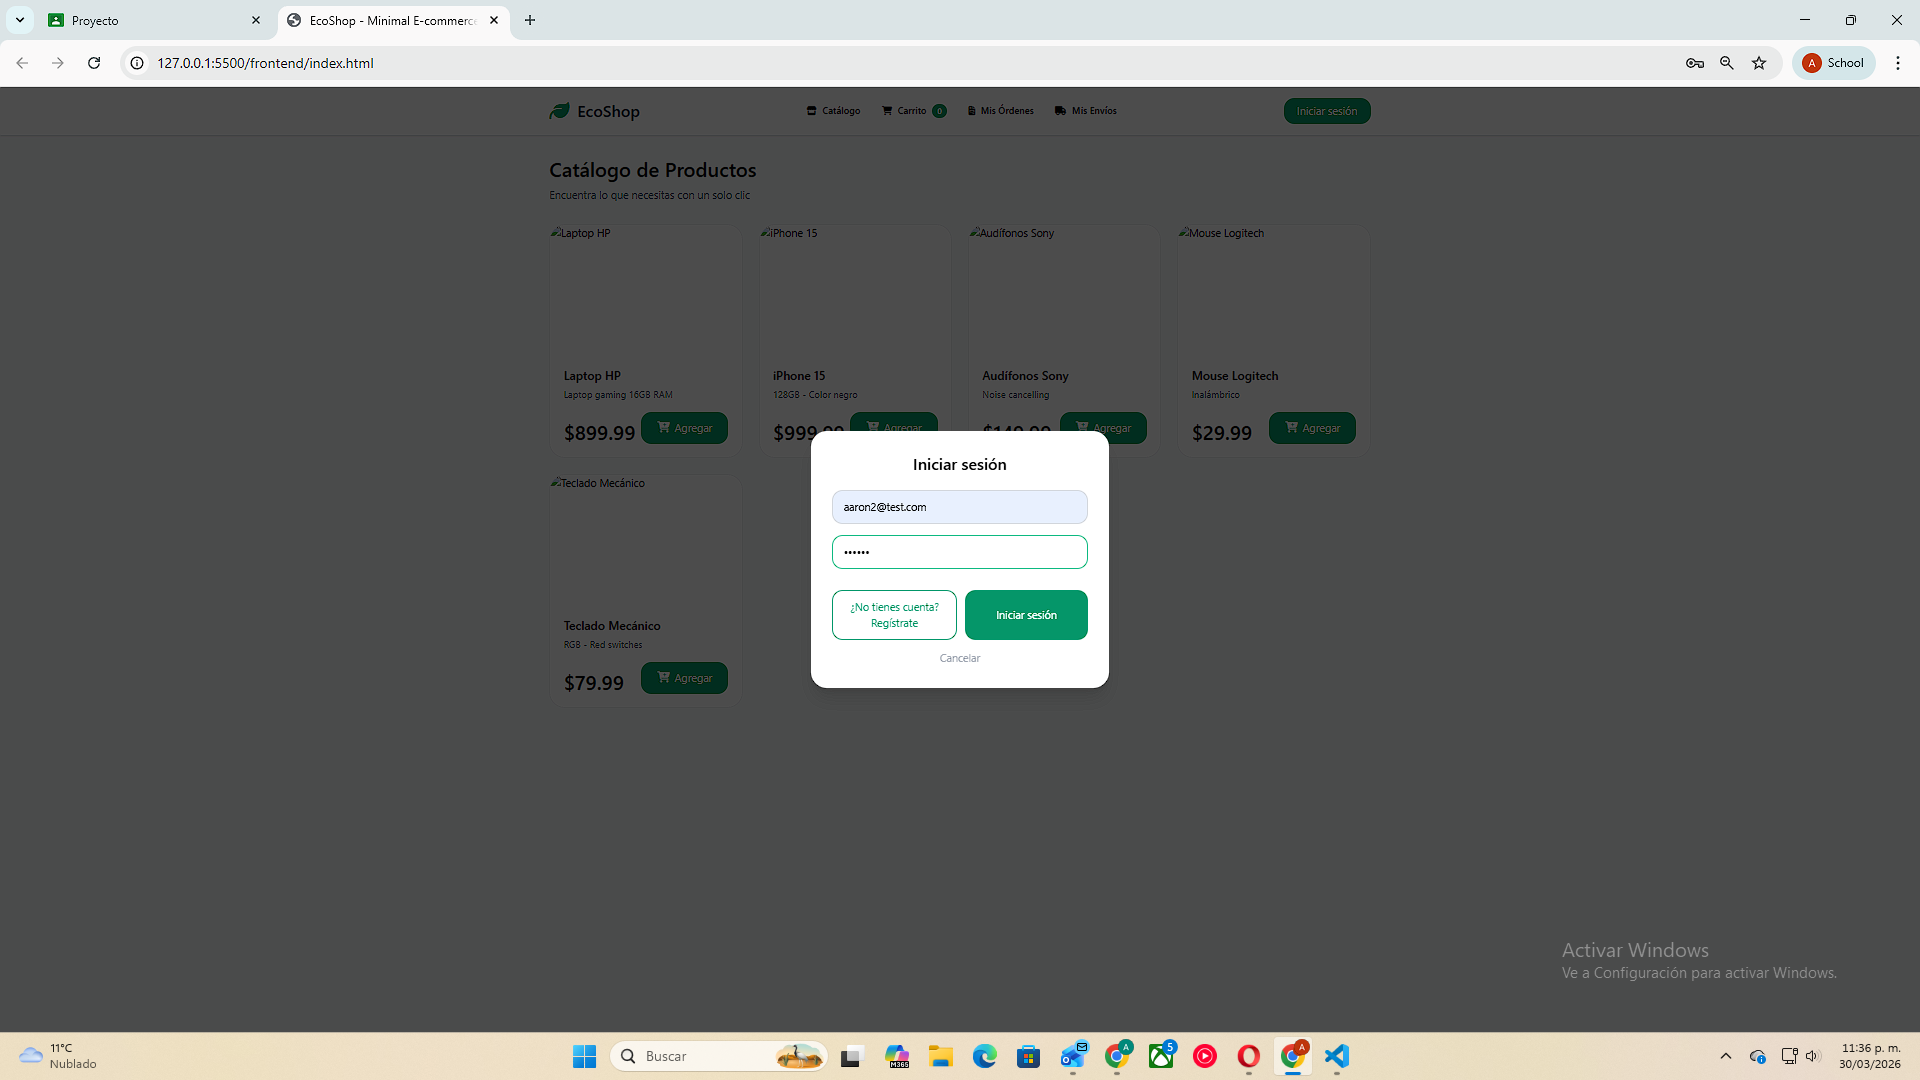
\includegraphics[width=0.85\textwidth]{imagenes/frontend_login.png}
    \caption{Pantalla de inicio de sesión y registro}
    \label{fig:frontend-login}
\end{figure}

\begin{figure}[H]
    \centering
    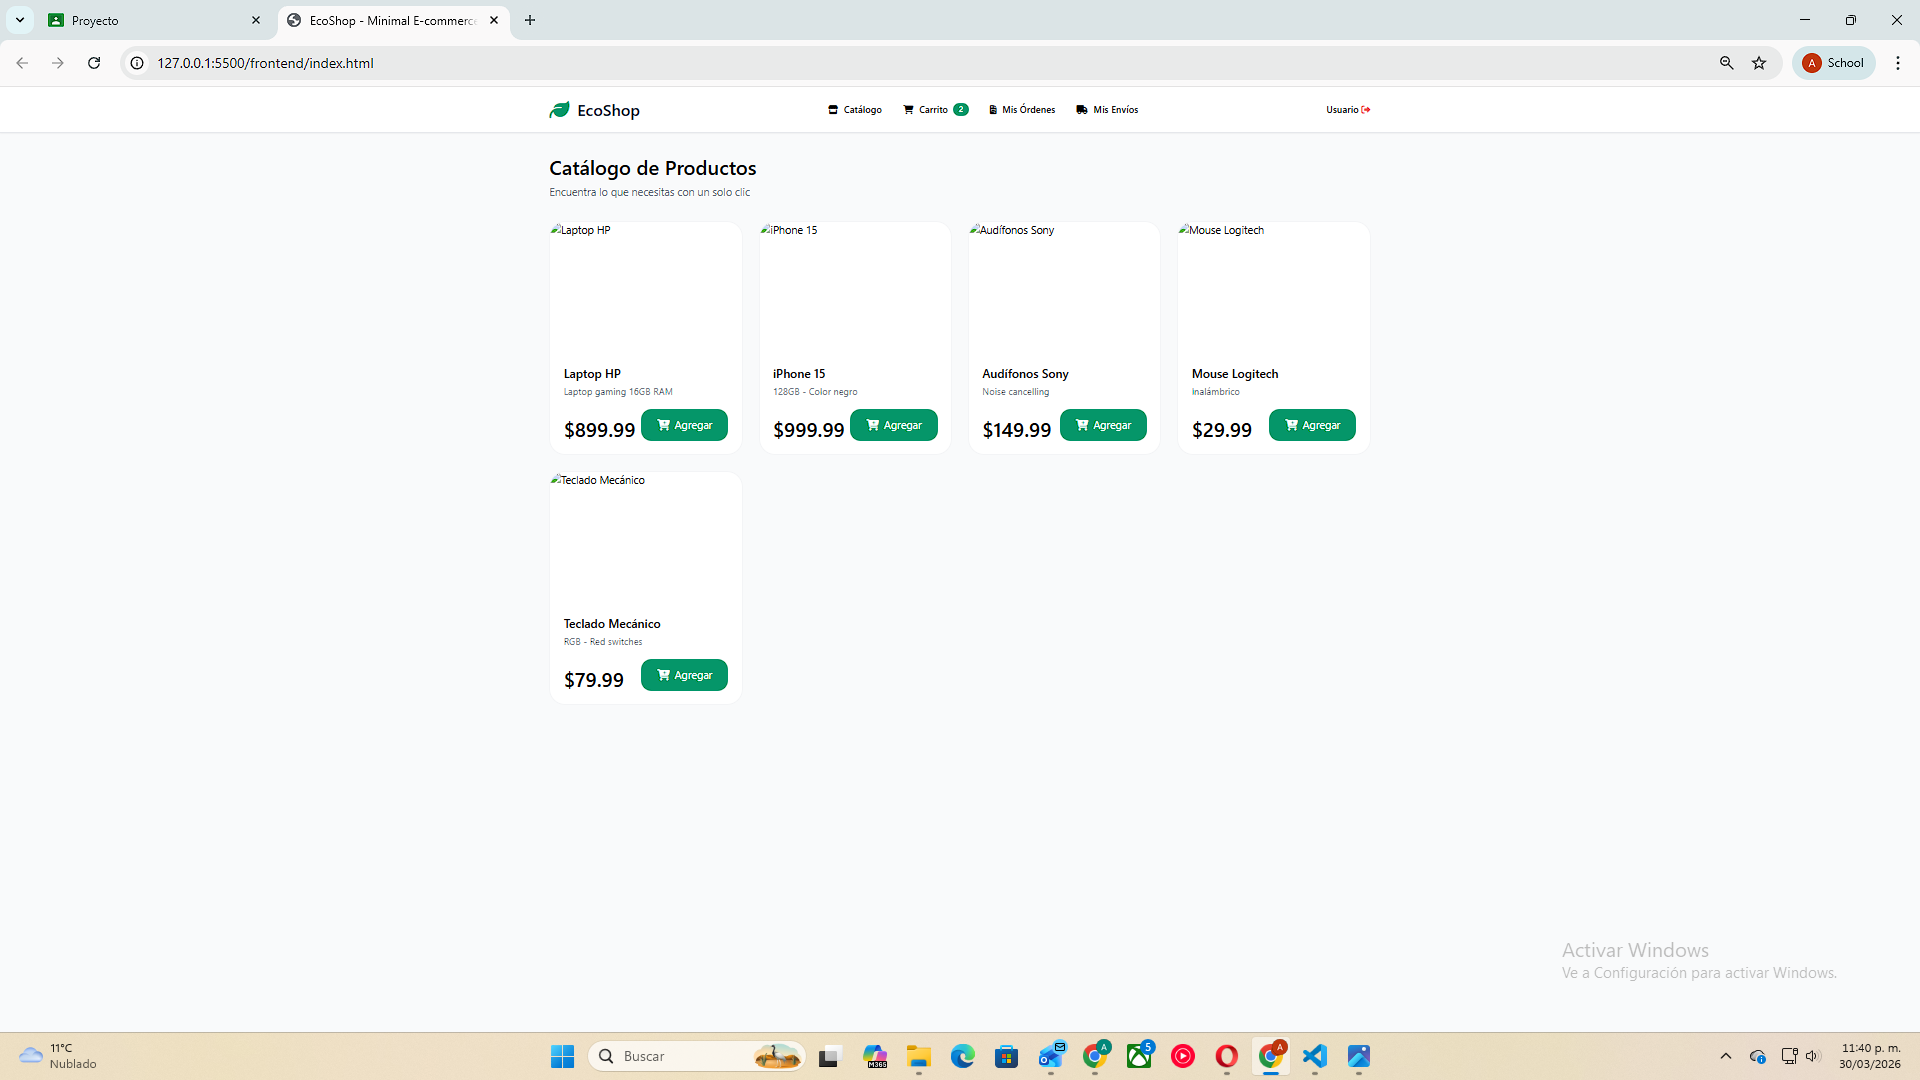
\includegraphics[width=0.85\textwidth]{imagenes/frontend_catalogo.png}
    \caption{Catálogo de productos cargado correctamente desde el Product Service}
    \label{fig:frontend-catalogo}
\end{figure}

\subsection{Flujo Completo de Compra}
Se validó exitosamente el flujo completo de una compra:

\begin{itemize}
    \item Inicio de sesión y obtención de token JWT.
    \item Navegación por el catálogo y adición de productos al carrito.
    \item Visualización y modificación del carrito de compras.
    \item Generación exitosa de una orden de compra.
    \item Creación automática del envío asociado.
\end{itemize}

\begin{figure}[H]
    \centering
    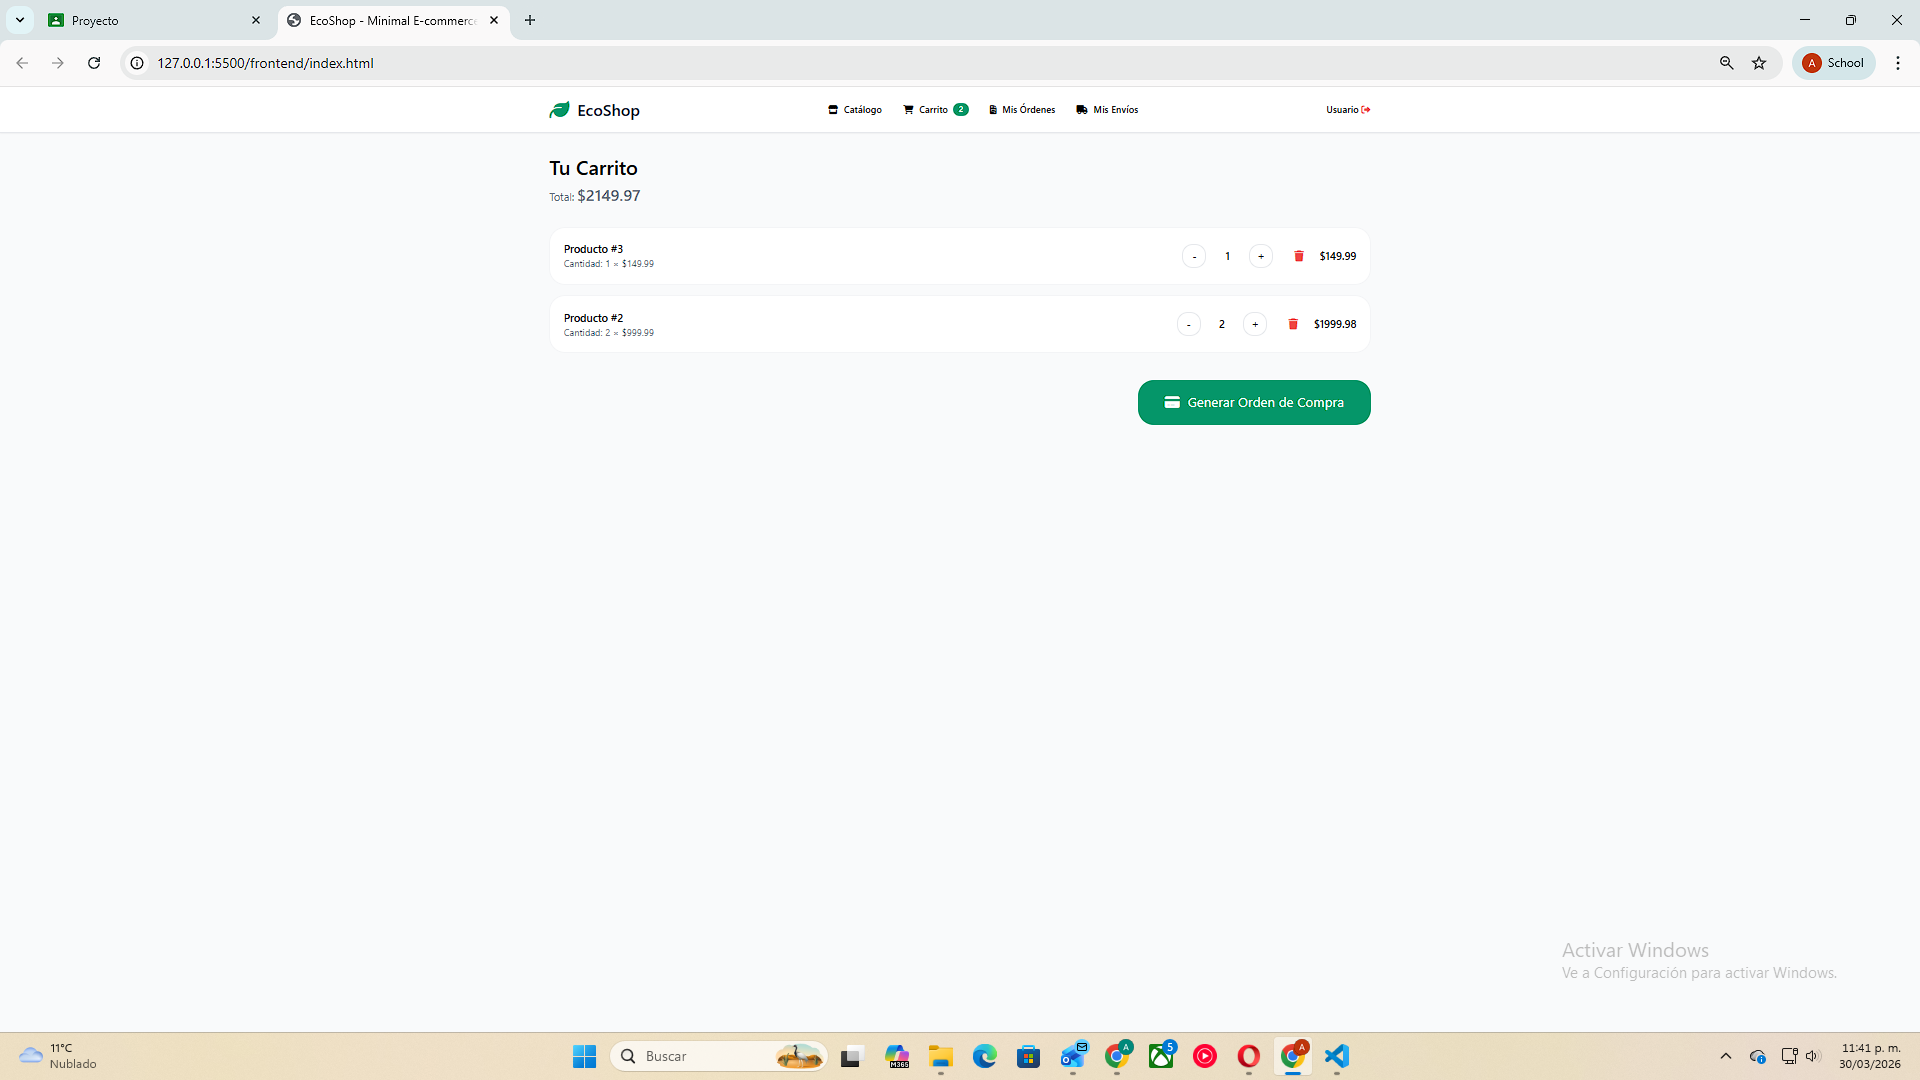
\includegraphics[width=0.85\textwidth]{imagenes/frontend_carrito.png}
    \caption{Carrito de compras con productos agregados}
    \label{fig:frontend-carrito}
\end{figure}

\begin{figure}[H]
    \centering
    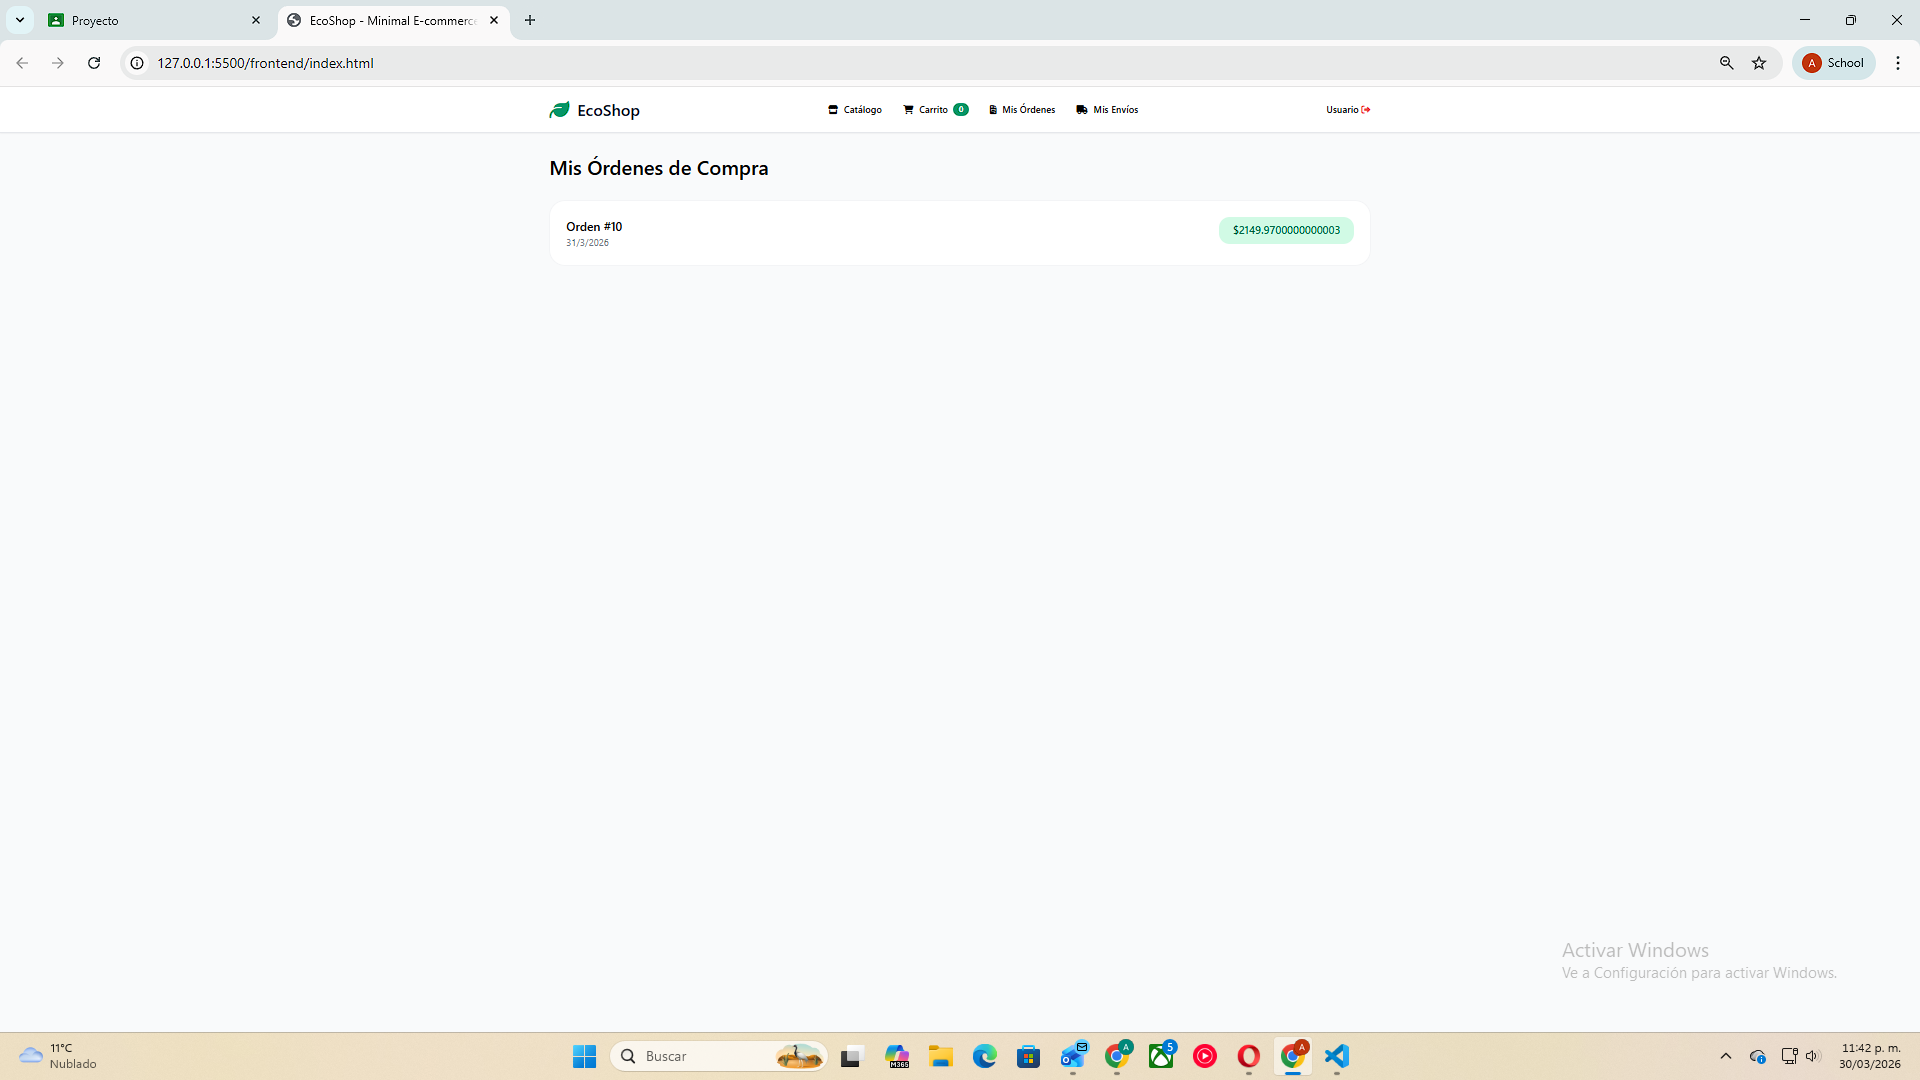
\includegraphics[width=0.85\textwidth]{imagenes/frontend_orden_generada.png}
    \caption{Confirmación de orden generada correctamente}
    \label{fig:frontend-orden}
\end{figure}

\subsection{Evidencia de Integración}
Las siguientes capturas muestran el correcto funcionamiento de las secciones "Mis Órdenes" y "Mis Envíos", demostrando que la comunicación entre el Order Service y el Shipment Service se ejecuta de forma adecuada.

\begin{figure}[H]
    \centering
    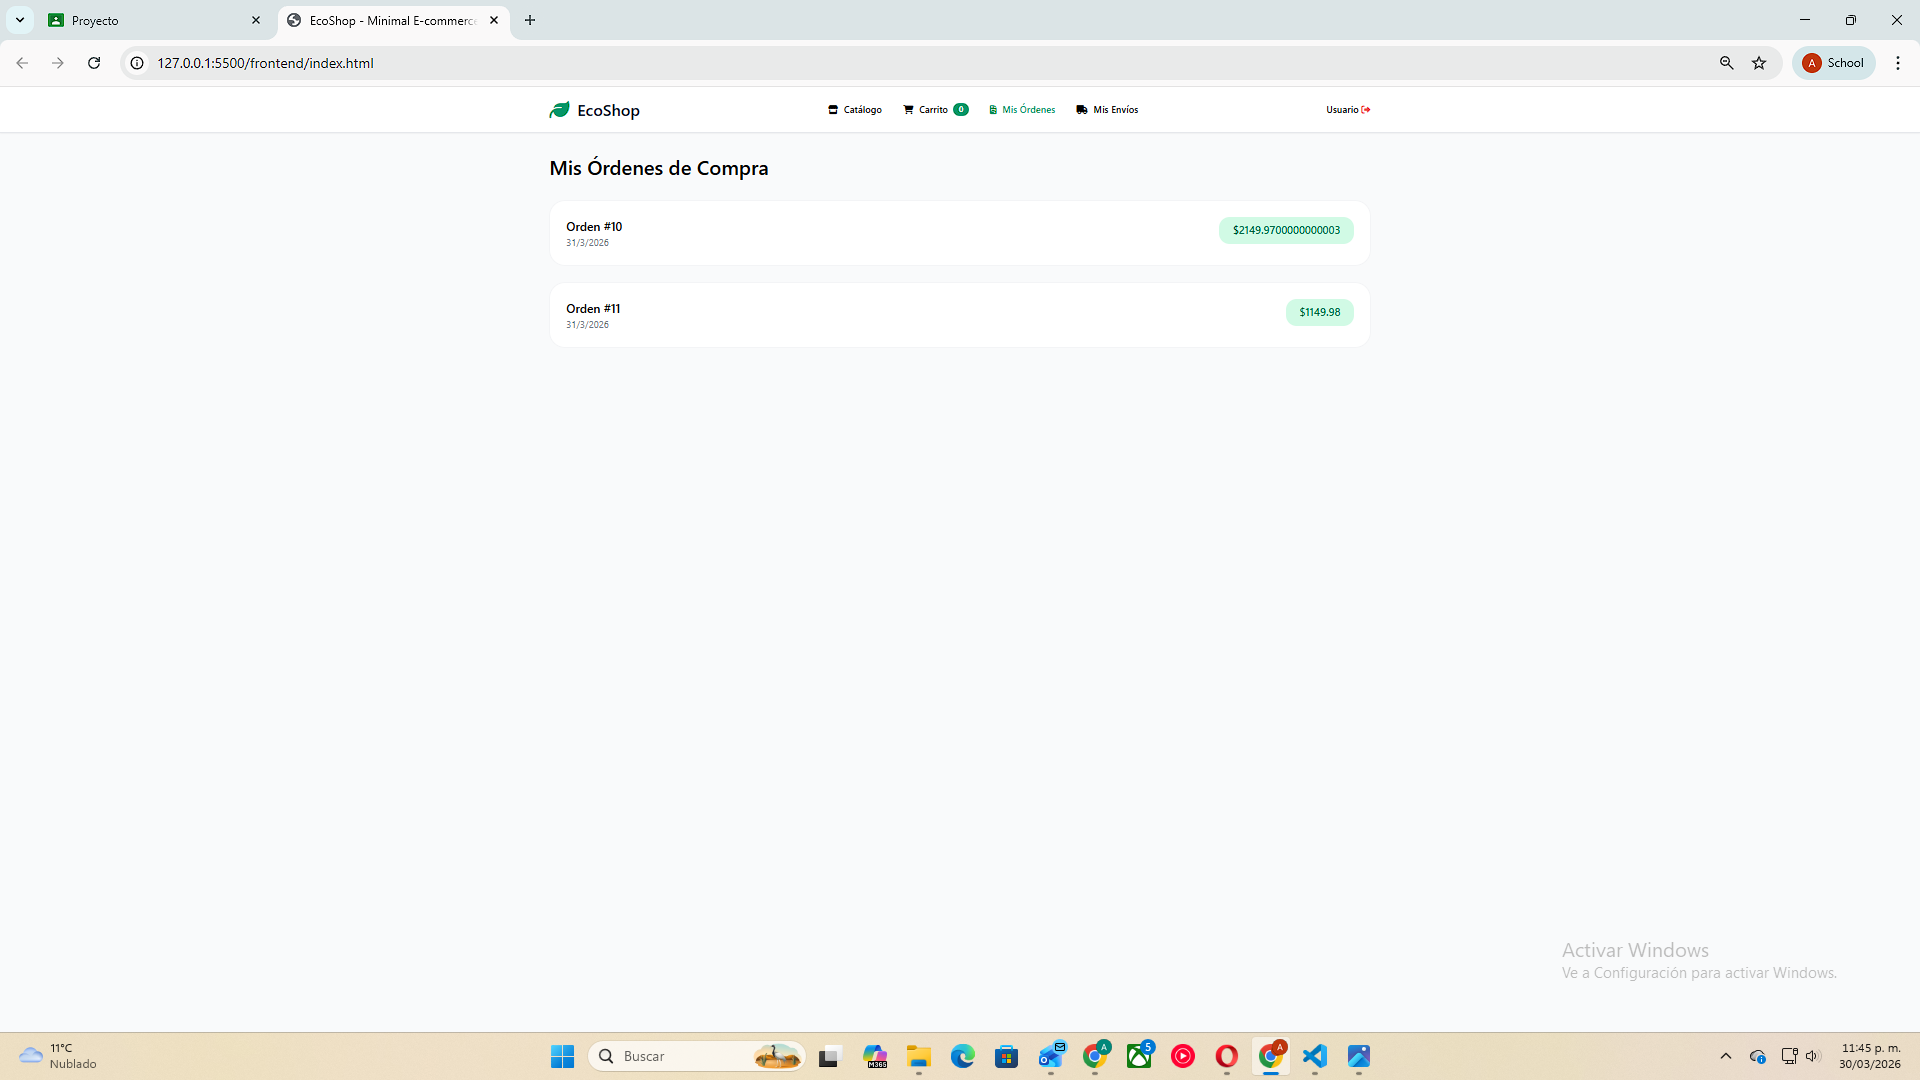
\includegraphics[width=0.85\textwidth]{imagenes/frontend_mis_ordenes.png}
    \caption{Pantalla de Mis Órdenes mostrando las órdenes generadas}
    \label{fig:mis-ordenes}
\end{figure}

\begin{figure}[H]
    \centering
    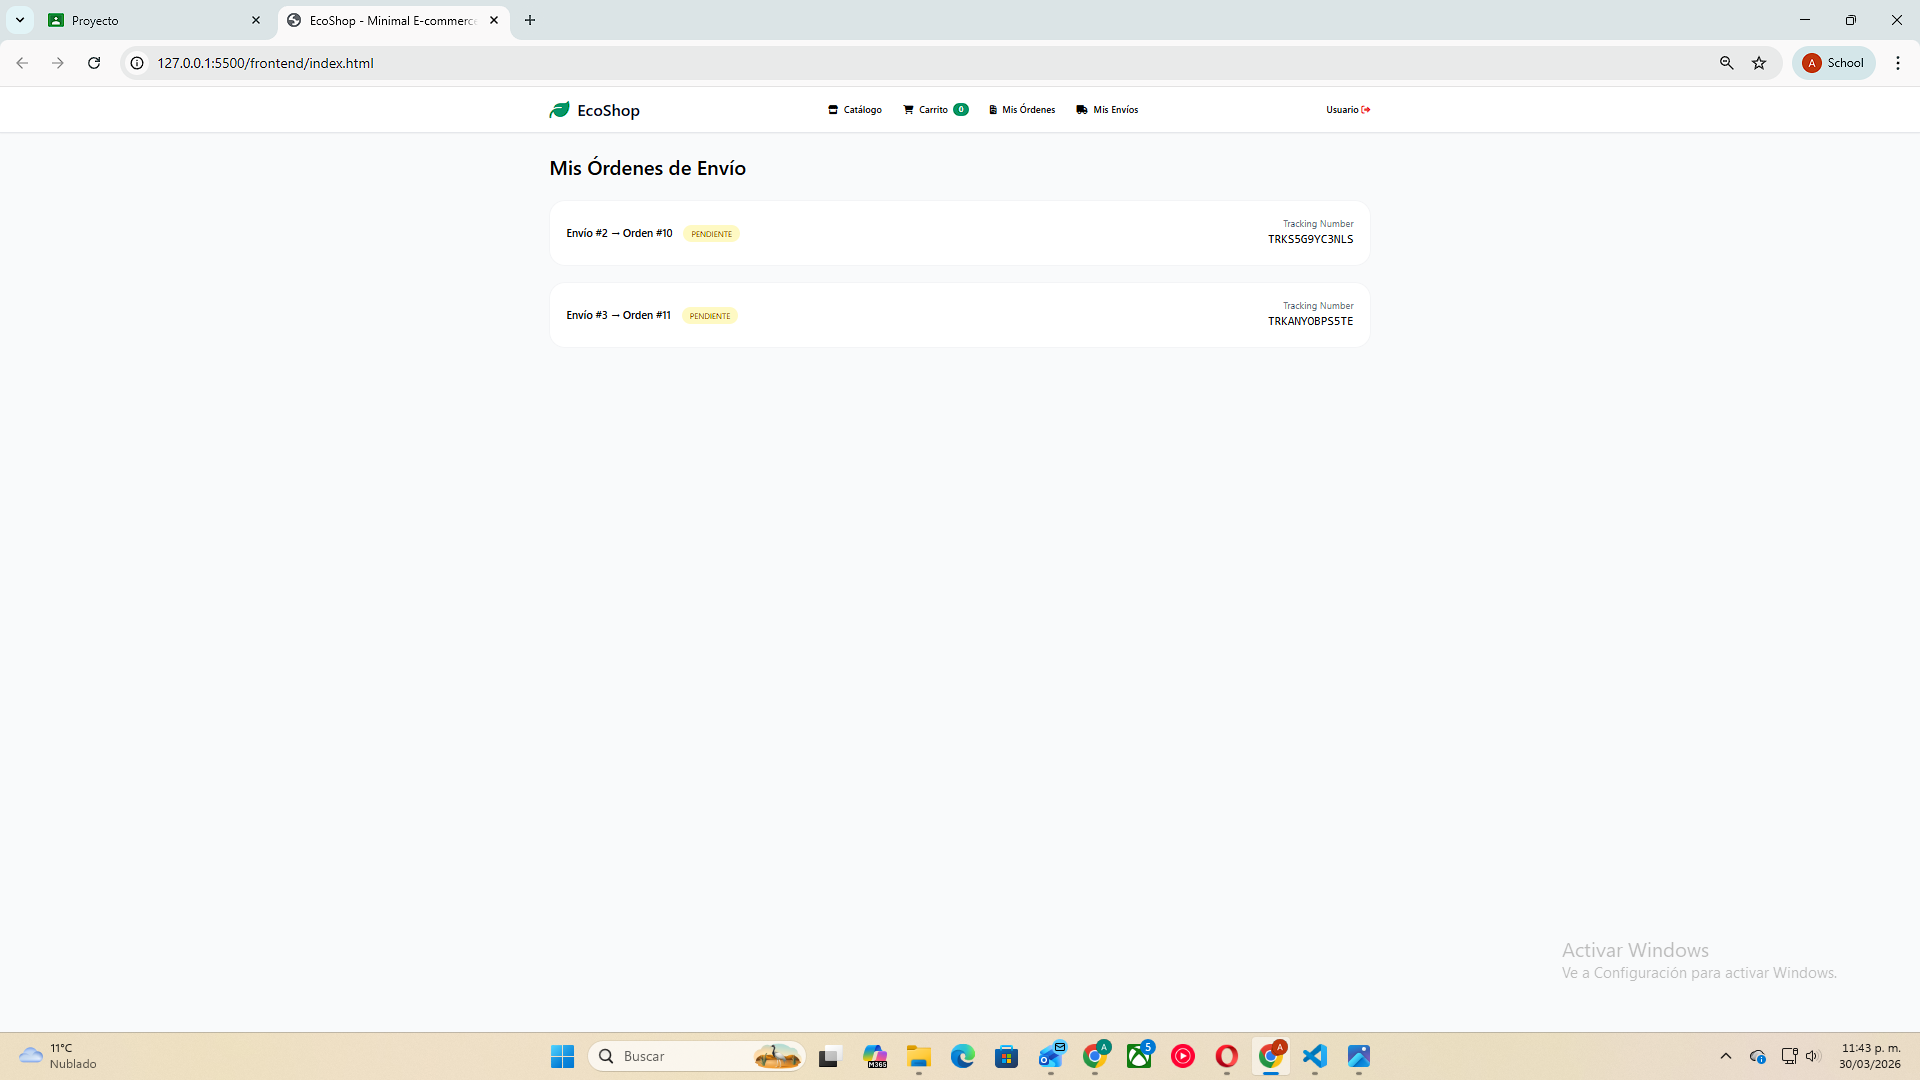
\includegraphics[width=0.85\textwidth]{imagenes/frontend_mis_envios.png}
    \caption{Pantalla de Mis Envíos con los envíos creados automáticamente}
    \label{fig:mis-envios}
\end{figure}

El sistema demuestra una integración estable y funcional entre el frontend y los cinco microservicios, cumpliendo con los requisitos de exposición, consumo y comunicación bidireccional entre servicios.


\section{Diagrama de Clases}

\begin{figure}[H]
    \centering
    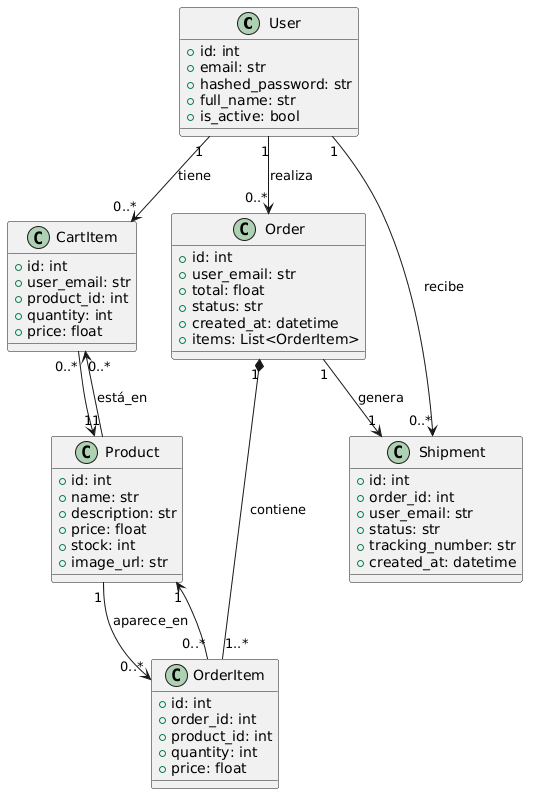
\includegraphics[width=0.95\textwidth]{imagenes/diagrama_clases.png}
    \caption{Diagrama de Clases del sistema de microservicios}
    \label{fig:clases}
\end{figure}

\section{Diagrama de Flujo}

\begin{figure}[H]
    \centering
    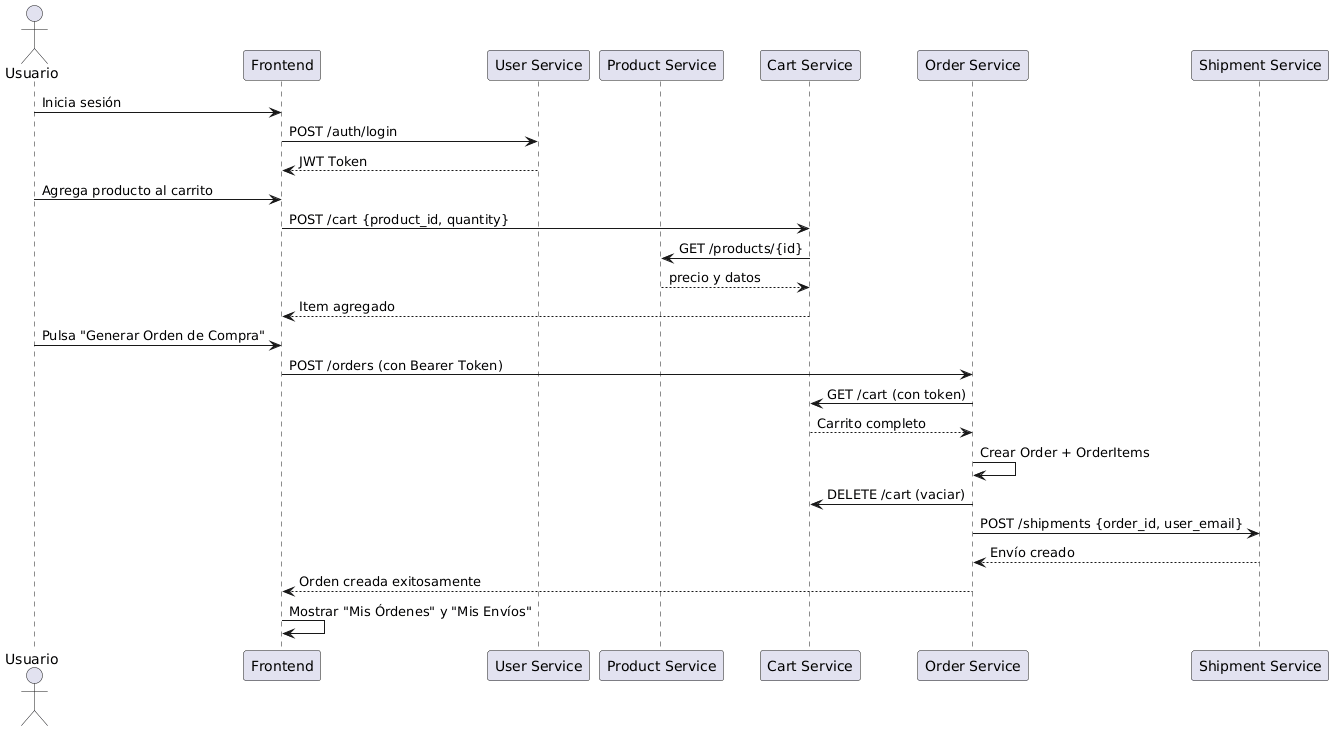
\includegraphics[width=0.95\textwidth]{imagenes/diagrama_de_flujo.png}
    \caption{Diagrama de Secuencia - Flujo de Compra}
    \label{fig:flujo}
\end{figure}

El flujo principal comienza con la autenticación del usuario, continúa con la selección de productos, agregarlos al carrito, y culmina con la creación de la orden y el envío automático.

\section{Arquitectura del Sistema}

\begin{figure}[H]
    \centering
    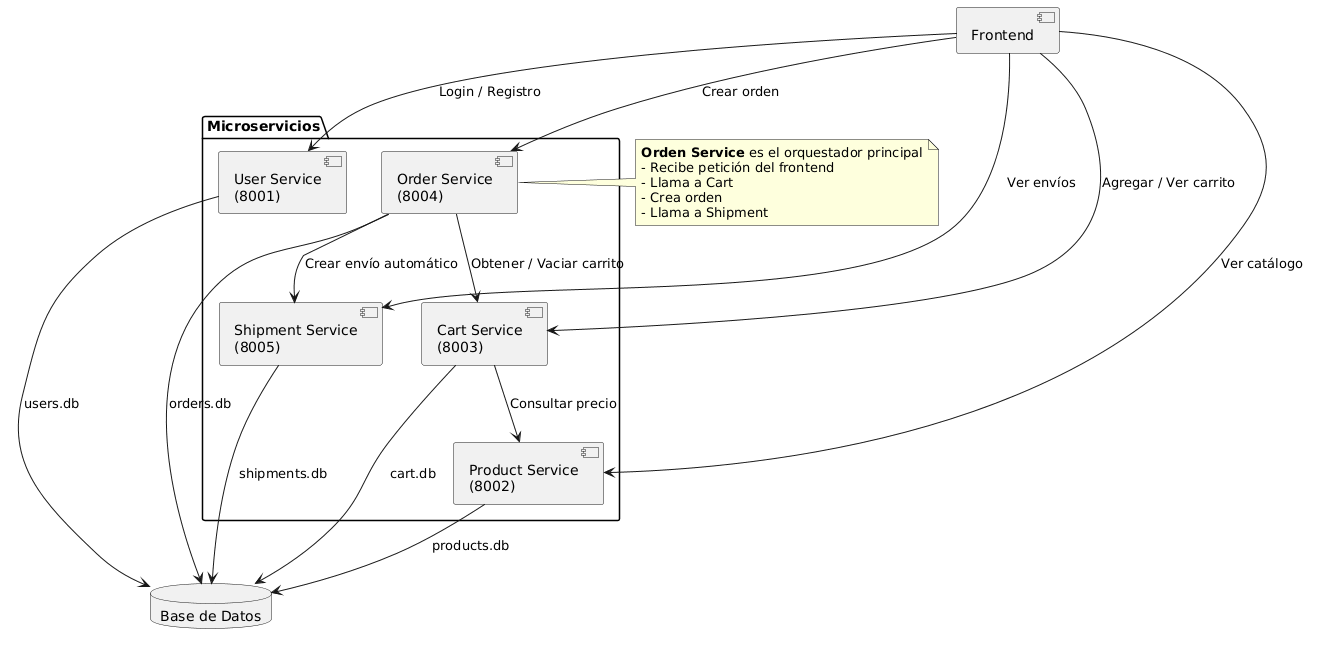
\includegraphics[width=0.95\textwidth]{imagenes/diagrama_de_arquitectura.png}
    \caption{Arquitectura General del Sistema}
    \label{fig:arquitectura}
\end{figure}

El sistema utiliza Docker Compose para orquestar los cinco microservicios y sus respectivas bases de datos SQLite. La comunicación entre servicios se realiza mediante HTTP/REST y todos comparten una red interna llamada \texttt{ecommerce-net}.

\section{Aprendizajes}

Durante el desarrollo de este proyecto se adquirieron los siguientes conocimientos:

\begin{itemize}
    \item Diseño e implementación de arquitecturas basadas en microservicios
    \item Comunicación entre servicios mediante APIs REST y manejo de tokens JWT
    \item Uso de Docker y Docker Compose para orquestación de contenedores
    \item Integración de FastAPI con SQLAlchemy y Pydantic
    \item Manejo de CORS y problemas comunes en aplicaciones distribuidas
    \item Buenas prácticas en el diseño de endpoints y validación de datos
    \item Depuración de errores en entornos multi-contenedor
\end{itemize}

\section{Conclusiones}

La implementación de este proyecto permitió comprender las ventajas y desafíos de trabajar con microservicios. Aunque aumenta la complejidad inicial en comparación con una aplicación monolítica, ofrece una mejor escalabilidad, mantenimiento y organización del código.

Se logró integrar exitosamente cinco servicios independientes con un frontend funcional, completando un flujo real de e-commerce. Este proyecto sirve como base sólida para futuras expansiones, como la incorporación de pagos, notificaciones y mayor robustez en la gestión de errores.

\vspace{1cm}
\textbf{Aaron Rodrigo Ramos Reyes} \\
\textbf{Eduardo Hernández Soto} \\
\textbf{Diego Sebastian Reyes García} \\
Cuajimalpa, Ciudad de México \\
\today

\end{document}